\documentclass{article}
\usepackage[pdftex]{graphicx}
\usepackage[margin=1in]{geometry}

\begin{document}

\title{Excerpt from Dialogues Concerning Two New Sciences [1638]}
\author{Galileo Galilei}
\date{Fall 2020}
\maketitle

\begin{center}
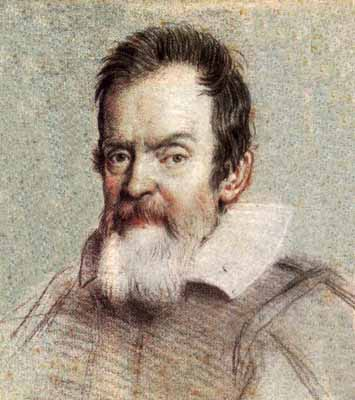
\includegraphics[width=3in]{images/Galileo_9.jpeg}
\end{center}

\begin{description}
\item[Salviati] An intellectual who seems to speak for Galileo 
\item[Sagredo]  A wealthy nobleman who is seeking truth. 
\item[Simplicio]  An Aristotelian philosopher who puts up ineffectual arguments for Salviati to knock down.
\end{description}


{\em Simp.}

Everyday experience shows that the propagation of light is instantaneous; for when we see a piece of artillery fired, at great distance, the flash reaches our eyes without lapse of time; but the sound reaches the ear only after a noticeable interval.

{\em Sagr.}

Well, Simplicio, the only thing I am able to infer from this familiar bit of experience is that sound, in reaching our ear, travels more slowly than light; it does not inform me whether the coming of the light is instantaneous or whether, although extremely rapid, it still occupies time. An observation of this kind tells us nothing more than one in which it is claimed that “As soon as the sun reaches the horizon its light reaches our eyes”; but who will assure me that these rays had not reached this limit earlier than they reached our vision?

{\em Salv.}

The small conclusiveness of these and other similar observations once led me to devise a method by which one might accurately ascertain whether illumination, i. e., the propagation of light, is really instantaneous. The fact that the speed of [88] sound is as high as it is, assures us that the motion of light cannot fail to be extraordinarily swift. The experiment which I devised was as follows:

Let each of two persons take a light contained in a lantern, or other receptacle, such that by the interposition of the hand, the one can shut off or admit the light to the vision of the other. Next let them stand opposite each other at a distance of a few cubits and practice until they acquire such skill in uncovering and occulting their lights that the instant one sees the light of his companion he will uncover his own. After a few trials the response will be so prompt that without sensible error [svario] the uncovering of one light is immediately followed by the uncovering of the other, so that as soon as one exposes his light he will instantly see that of the other. Having acquired skill at this short distance let the two experimenters, equipped as before, take up positions separated by a distance of two or three miles and let them perform the same experiment at night, noting carefully whether the exposures and occultations occur in the same manner as at short distances; if they do, we may safely conclude that the propagation of light is instantaneous; but if time is required at a distance of three miles which, considering the going of one light and the coming of the other, really amounts to six, then the delay ought to be easily observable. If the experiment is to be made at still greater distances, say eight or ten miles, telescopes may be employed, each observer adjusting one for himself at the place where he is to make the experiment at night; then although the lights are not large and are therefore invisible to the naked eye at so great a distance, they can readily be covered and uncovered since by aid of the telescopes, once adjusted and fixed, they will become easily visible.

{\em Sagr.}

This experiment strikes me as a clever and reliable invention. But tell us what you conclude from the results.

{\em Salv.}

In fact I have tried the experiment only at a short distance, less than a mile, from which I have not been able to ascertain with certainty whether the appearance of the opposite light was instantaneous or not; but if not instantaneous it is extraordinarily rapid---I should call it momentary; and for the present I should compare it to motion which we see in the lightning flash between clouds eight or ten miles distant from us. We see the beginning of this light---I might say its head and[89] source---located at a particular place among the clouds; but it immediately spreads to the surrounding ones, which seems to be an argument that at least some time is required for propagation; for if the illumination were instantaneous and not gradual, we should not be able to distinguish its origin---its center, so to speak---from its outlying portions. What a sea we are gradually slipping into without knowing it! With vacua and infinities and indivisibles and instantaneous motions, shall we ever be able, even by means of a thousand discussions, to reach dry land?

{\em Sagr.}

Really these matters lie far beyond our grasp. Just think; when we seek the infinite among numbers we find it in unity; that which is ever divisible is derived from indivisibles; the vacuum is found inseparably connected with the plenum; indeed the views commonly held concerning the nature of these matters are so reversed that even the circumference of a circle turns out to be an infinite straight line, a fact which, if my memory serves me correctly, you, Salviati, were intending to demonstrate geometrically. Please therefore proceed without further digression.

\end{document}